%\section{BEO Representativeness}
%%%%%%%%%%%%%%%%%%%%%%%%%%%%%%%%%%%%%%%%%%%%%%%%%%%%%%%%%%%%%%%%%%%%%%%%%%%%%%%
\begin{frame}
 \frametitle{Barrow Environmental Observatory (BEO)}
 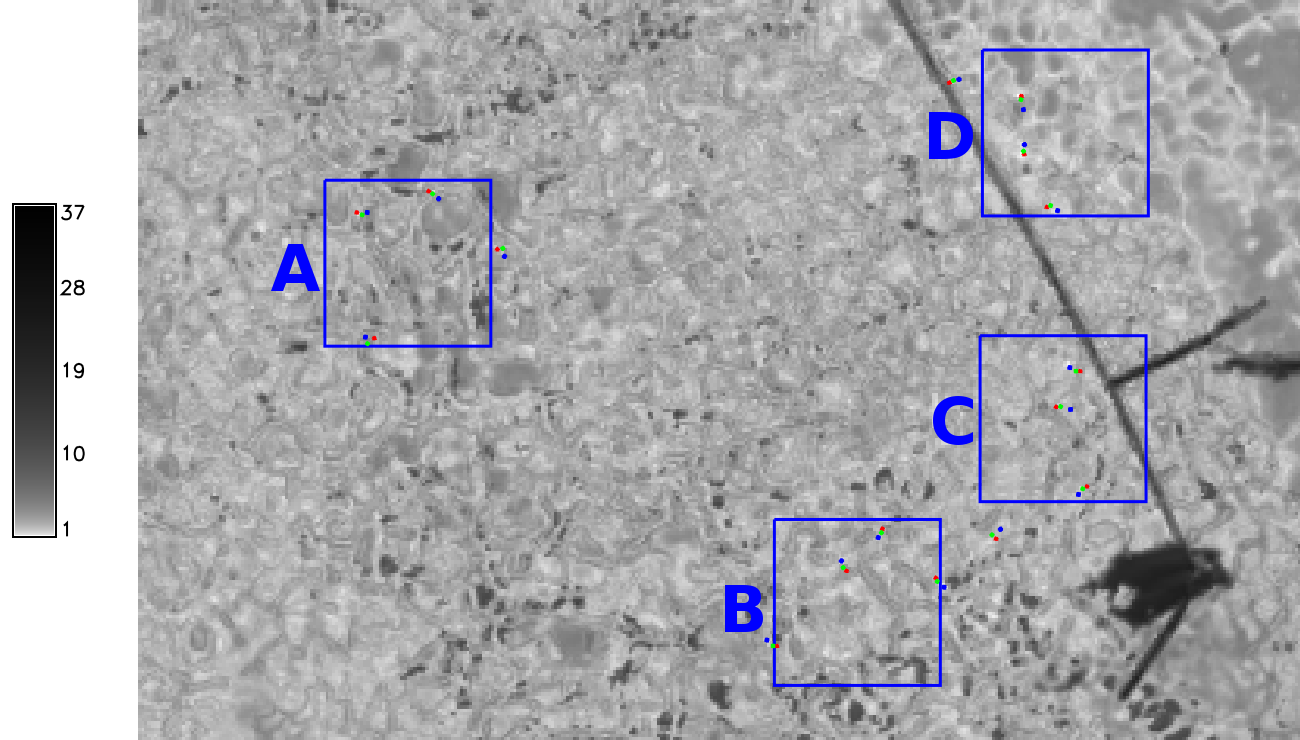
\includegraphics[width=0.47\textwidth]{beo_figures/ABCDv2.png}
 \hfill
 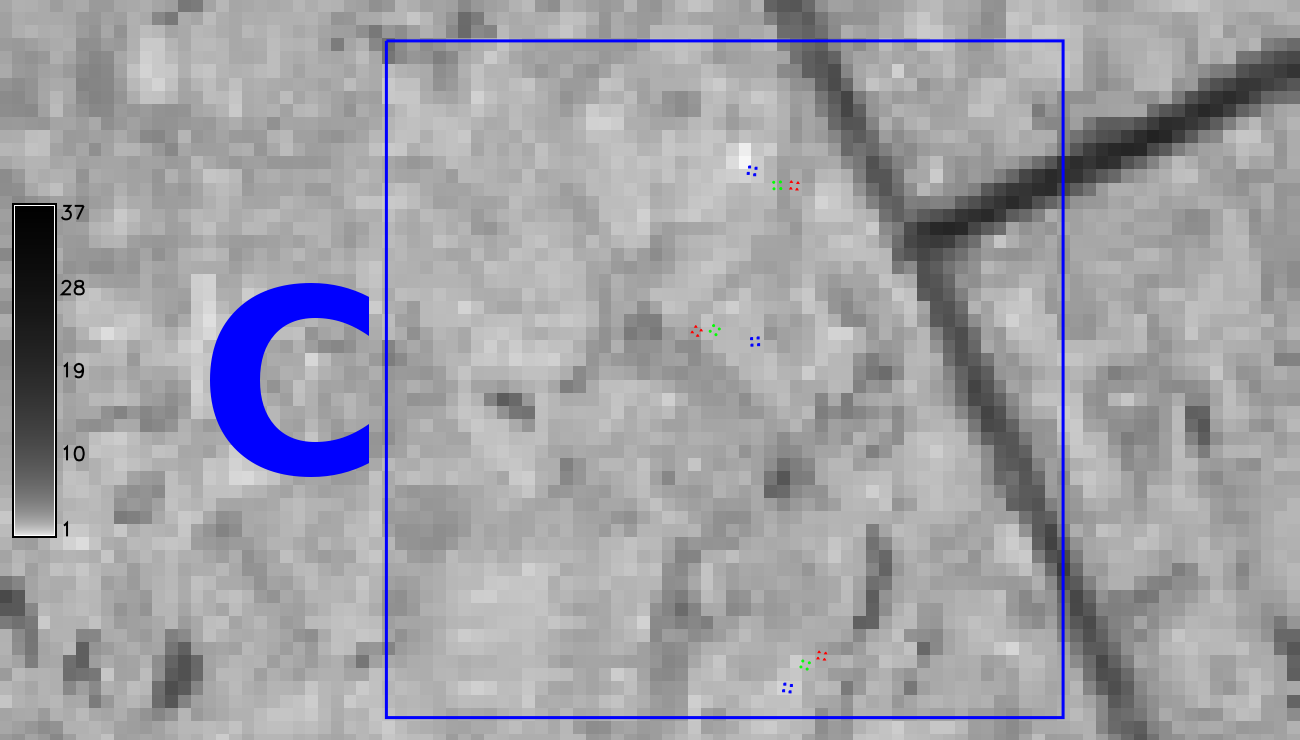
\includegraphics[width=0.47\textwidth]{beo_figures/Cv2.png} \\
 \vbox{\scriptsize\hfill (Kumar et al., in prep)}

\medskip
Representativeness map for vegetation sampling points for A, B, C, and D
sampling area (left) and zoomed in on the C samping area (right) developed
from WorldView2 satellite images for the year 2010 and LiDAR data.

\medskip
Vegetation sampling locations represent polygon troughs (red), edges
(green), and centers (blue).

\end{frame}
%%%%%%%%%%%%%%%%%%%%%%%%%%%%%%%%%%%%%%%%%%%%%%%%%%%%%%%%%%%%%%%%%%%%%%%%%%%%%%%

%%%%%%%%%%%%%%%%%%%%%%%%%%%%%%%%%%%%%%%%%%%%%%%%%%%%%%%%%%%%%%%%%%%%%%%%%%%%%%%
\begin{frame}

\vskip-0.15in
\begin{figure}
 {\centering\footnotesize
 \hfil
 \subfigure[dry tundra gramanoid]{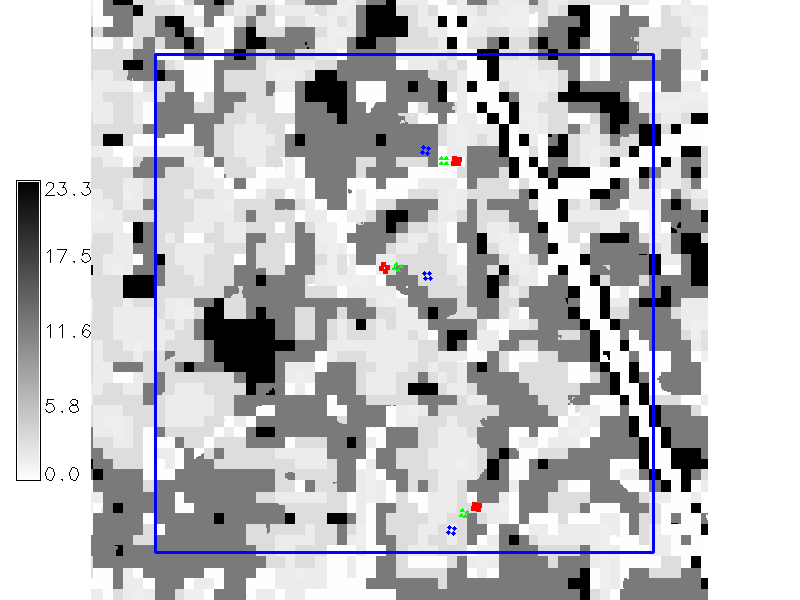
\includegraphics[width=0.40\textwidth]{beo_figures/areac_dry_tundra_graminoid.png}\label{fig:areac_dry_tundra_graminoid}}
 \hfil
 \subfigure[forb]{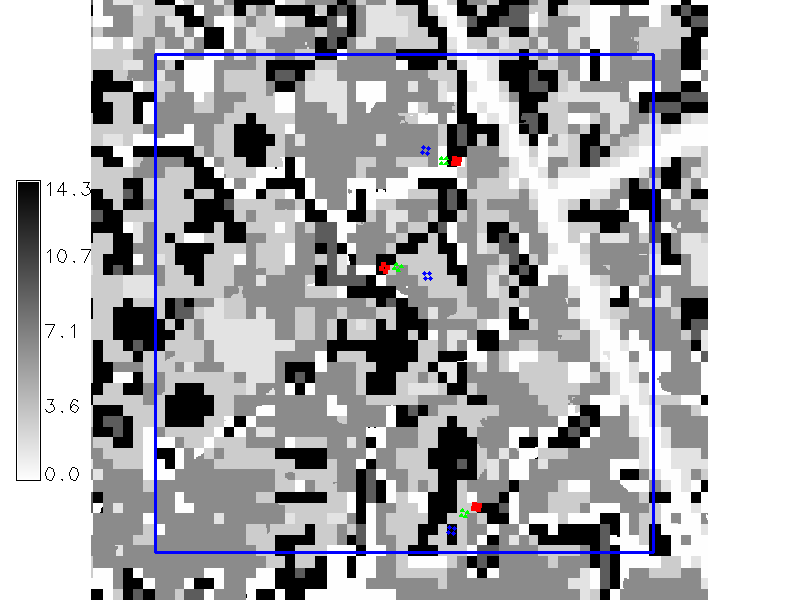
\includegraphics[width=0.40\textwidth]{beo_figures/areac_forb.png}\label{fig:areac_forb}}
 \hfil \\
 \hfil
 \subfigure[lichen]{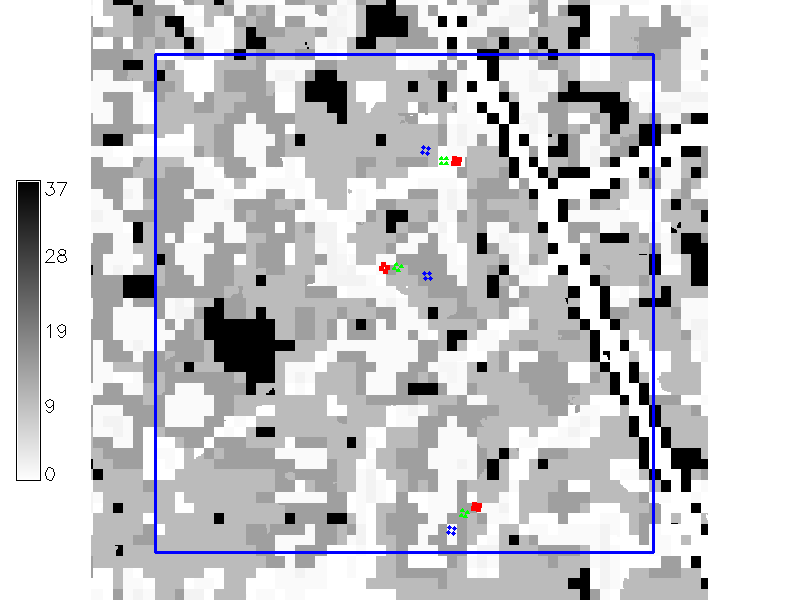
\includegraphics[width=0.40\textwidth]{beo_figures/areac_lichen.png}\label{fig:areac_lichen}}
 \hfil
 \subfigure[moss]{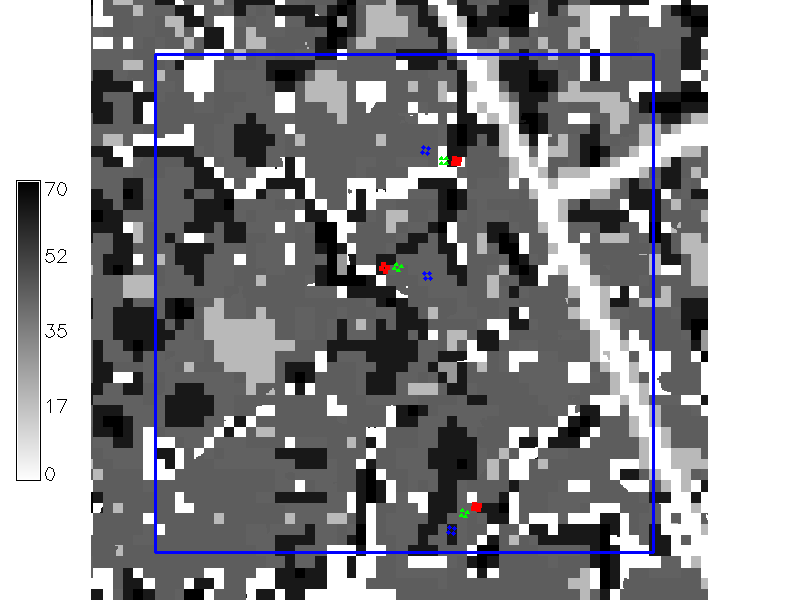
\includegraphics[width=0.40\textwidth]{beo_figures/areac_moss.png}\label{fig:areac_moss}}
 \hfil \\
 \vskip-0.10in\vbox{\scriptsize\hfill (Kumar et al., in prep)}
 }
% \caption{Using WorldView2 satellite imagery and LiDAR data, plant
% functional type (PFT) distributions were scaled up to each sampling
% area based on their proportion at vegetation sampling locations.
% Four such PFT distribution maps are shown for area C.}
 \label{fig:areac_pfts}
\end{figure}

\vskip-0.15in
Example plant functional type (PFT) distributions scaled up from vegetation sampling locations.

\end{frame}
%%%%%%%%%%%%%%%%%%%%%%%%%%%%%%%%%%%%%%%%%%%%%%%%%%%%%%%%%%%%%%%%%%%%%%%%%%%%%%%
